\chapter{Stochastic Optimization}


\section{Simulated Annealing}
The goal of Simulated Annealing(SA) is to find a state $\boldsymbol{s}$ that minimize  a cost function $E_{T(\boldsymbol{s})}$ where $s_i \in \boldsymbol{s}$ is a discrete variable.

$$
\boldsymbol{s}^* = \underset{\boldsymbol{s}}{\text{argmin}} E_{T(\boldsymbol{s})}
$$

\begin{algorithm}[H]
\caption{Simulated Annealing}
 \KwData{$\boldsymbol{s}_0, \tau, M, \beta_0$ }
 \For{annealing loop, $t=1,2,..$}{
  $\boldsymbol{s}_t = \boldsymbol{s}_{t-1}$ 
  
  \For{$M $iterations}{
  		$\boldsymbol{s}' =$ do local permutation from $\boldsymbol{s}_t$ \;
  		$\Delta E = E_{\boldsymbol{s}'} - E_{\boldsymbol{s}_t}$ \;
  		switch to $\boldsymbol{s}_t$ to $\boldsymbol{s}'$ with probability $W = \frac{1}{1+\exp{(\beta_t \Delta E)}}$
}
$\beta_{t+1} = \tau \beta_t \hspace{0.5cm} \tau \in [1.01 - ... ]$

 }
\end{algorithm}

where $\beta = 1 / \tau $ and $M \approx 2000$. Ideally, we want  $\beta_t = \ln t$ but this is too slow in practice.

Influence of $T$ and $\beta$ to transition probability $W$.
\begin{itemize}
	\item $\downarrow T \uparrow  \beta $ : $W$ changes \textbf{dramatically} when $\Delta E$ has a slight change.
	\item $\uparrow T \downarrow  \beta $ : $W$ \textbf{barely} changes  when $\Delta E$ has a huge change.
\end{itemize}

\begin{figure}[hbt]
	\center
  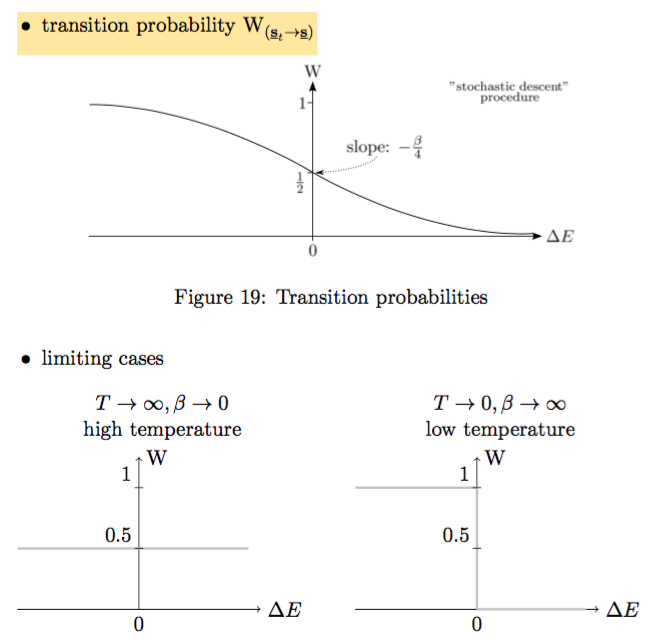
\includegraphics[width=0.8\textwidth]{figures/so-transition-probability}
  \caption{Transition Probability}
  \label{fig:so-transition-probability}
\end{figure}


\section{The Gibbs Distribution}
% SA : what is markov property?
If we fix $T$ or $\beta$ at a specific value,  this results in a stochastic process with Markov property\footnote{what is this property?}. Hence $P_{(\boldsymbol{s})}$ converges to a stationary distribution as $t \rightarrow \infty$.

$$
\lim_{t' \rightarrow \infty }  \prod(\boldsymbol{s}, t') = P_{(\boldsymbol{s})} \hspace{0.5cm}
$$

With \textbf{Detailed Balance} assumption which states as follow :

$$
P_{(\boldsymbol{s})} W_{\boldsymbol{s} \rightarrow \boldsymbol{s}' } = P_{(\boldsymbol{s}')} W_{\boldsymbol{s}' \rightarrow \boldsymbol{s} }
$$

We can find $P_{(\boldsymbol{s})} $ analytically : 

\begin{align*}
	\frac{P_{(\boldsymbol{s})}}{P_{(\boldsymbol{s}')}} &= \frac{W_{\boldsymbol{s}' \rightarrow \boldsymbol{s} }}{W_{\boldsymbol{s} \rightarrow \boldsymbol{s}' }} \\
	&= \frac{  1 + \exp{( \beta(E_{\boldsymbol{s}'} - E_{\boldsymbol{s}})   )} }{  1 + \exp{( \beta(E_{\boldsymbol{s}} - E_{\boldsymbol{s}'}) )  } } \\
	&= \frac{  1 + \exp{( \beta \Delta E} ) }{  1 + \exp{ (- \beta \Delta E)  } } \\
	&= \exp{( \beta \Delta E ) }
\end{align*}

To fulfill this condition, we need $P_{(\boldsymbol{s})}$ to be a Gibbs-Boltzmann Distribution
\begin{align*}
	P_{(\boldsymbol{s})} = \frac{1}{Z} \exp{( -\beta E_{\boldsymbol{s}} )} 
\end{align*}
where $Z = \sum_{\boldsymbol{s}} \exp{(-\beta E_{\boldsymbol{s}})}$.

\section{Mean-field Annealing}
As we know that $P_{(\boldsymbol{s})}$ has an analytic solution, we can exploit this knowledge to make the optimization faster, but estimate $P_{(\boldsymbol{s})}$ is difficult and its moment doesn't have analytic solution. 

To alleviate the problem, we will choose a distribution $Q_{(\boldsymbol{s})}$ that approximates $P_{(\boldsymbol{s})}$. Formally, $Q_{(\boldsymbol{s})}$ is a factorizing distribution that $E_Q$ is a linear combination of $s_k$. 

\begin{align*}
	Q_{\boldsymbol{s}} &= \frac{1}{Z_Q} \exp{ \Bigg ( - \beta E_Q  \Bigg )}   \\
	&= \frac{1}{Z_Q} \exp{ \Bigg ( - \beta \sum_{k} e_k s_k  \Bigg )}  
\end{align*}

$e_k$ is the mean field that parameterizes family of distributions. As $\beta \rightarrow \infty$, the first moment $\langle \boldsymbol{s} \rangle_{Q}$ well characterizes the distributions. For example, it will peak at the location of optimum value.

For factorized distribution, 

\begin{align*}
	Q_{(\boldsymbol{s})} = \prod_k Q_{(\boldsymbol{s}_k)}
\end{align*}

and the moment of 2 independent variables $f_{(\boldsymbol{s} / s_l) }$ and $g_{(s_l)}$ of $\boldsymbol{s}$ can be computed as follows :

\begin{align*}
	\langle  f_{(\boldsymbol{s} / s_l) } g_{(s_l)}  \rangle &= \frac{1}{Z_Q} \sum_{\boldsymbol{s}} f_{(\boldsymbol{s} / s_l) } g_{(s_l)} \exp{ \Bigg (  -\beta \sum_{ s_k \in \boldsymbol{s}}  e_k s_k \Bigg ) }  \\
	&= \frac{1}{Z_Q} \Bigg [  f_{(\boldsymbol{s} / s_l)} g_{(s_{l,i})}  \exp{ \bigg ( -\beta \sum_{ s_k \in \boldsymbol{s} / s_l}  e_k s_k \bigg ) \exp{ \bigg (  -\beta e_l s_{l,i} \bigg ) }+  \dots  }                            \Bigg ] \\
	&= \frac{1}{Z_Q} \Bigg [  f_{(\boldsymbol{s} / s_l)}  \exp{ \bigg ( -\beta \sum_{ s_k \in \boldsymbol{s} / s_l}  e_k s_k \bigg ) \bigg( \sum_{s_{l,i} \in s_l} g_{s_{l,i}}  \exp{ \bigg (  -\beta e_l s_{l,i} \bigg ) } \bigg) +  \dots  }                            \Bigg ] \\
	&= \frac{1}{Z_Q} \Bigg [ \sum_{\boldsymbol{s} / s_l}  f_{(\boldsymbol{s} / s_l) }  \exp{ \bigg (  -\beta \sum_{ s_k \in \boldsymbol{s} / s_l}  e_k s_k \bigg ) }  \Bigg ] \Bigg[  \sum_{s_{l,i} \in s_l} g_{(s_{l,i})} \exp{ \bigg ( -\beta e_l s_{l,i} \bigg)}\Bigg] \\
	&= \frac{1}{Z_Q} \Bigg [ \sum_{\boldsymbol{s} / s_l}  f_{(\boldsymbol{s} / s_l) }  \exp{ \bigg (  -\beta \sum_{ s_k \in \boldsymbol{s} / s_l}  e_k s_k \bigg ) }  \Bigg ] \frac{ \sum_{s_{l,i} \in s_l} \exp{ \bigg ( -\beta e_l s_{l,i} \bigg)}}{ \sum_{s_{l,i} \in s_l} \exp{ \bigg ( -\beta e_l s_{l,i} \bigg)} }      \Bigg[  \sum_{s_{l,i} \in s_l} g_{(s_{l,i})} \exp{ \bigg ( -\beta e_l s_{l,i} \bigg)}\Bigg] \\
	&= \underbrace{ \frac{1}{Z_Q} \Bigg [ \sum_{\boldsymbol{s} / s_l}  f_{(\boldsymbol{s} / s_l) }  \exp{ \bigg (  -\beta \sum_{ s_k \in \boldsymbol{s} }  e_k s_k \bigg ) }  \Bigg ] }_{ \langle f_{(\boldsymbol{s} / s_l} \rangle_{Q} } \underbrace{\frac{1}{ \sum_{s_{l,i} \in s_l} \exp{ \bigg ( -\beta e_l s_{l,i} \bigg)} }      \Bigg[  \sum_{s_{l,i} \in s_l} g_{(s_{l,i})} \exp{ \bigg ( -\beta e_l s_{l,i} \bigg)}\Bigg]}_{\langle g_{(s_l)} \rangle_{Q} } \\
\end{align*}

Therefore,  
$$
\langle s_l \rangle_Q = \frac{ \sum_{s_{l,i} \in s_l} s_{l,i} \exp{ \bigg ( -\beta e_l s_{l,i} \bigg)} }{ \sum_{s_{l,i} \in s_l} \exp{ \bigg ( -\beta e_l s_{l,i} \bigg)} } 
$$


\subsubsection{The mean-field approximation}
\begin{itemize}
	\item True Distribution : \ $P_{(\boldsymbol{s})} = \frac{1}{Z}\exp{(-\beta E_p)}$
	\item Approximation Distribution : \ $Q_{(\boldsymbol{s})} = \frac{1}{Z}\exp{(-\beta \sum_{k} e_k s_k )}$ and $e_k$ are mean fields which we shall find.
\end{itemize}
To find $e_k$, we minimize Kullback-Leibler Divergence as follow : 

\begin{align*}
	D_{KL}(Q||P) &= \sum_{\boldsymbol{s}} Q_{(\boldsymbol{s})} \ln \frac{Q_{(\boldsymbol{s})}}{P_{(\boldsymbol{s})}} \\
	&\stackrel{!}{=} \min 
\end{align*}


To find $e_l$, we do $\frac{\partial D_{KL} }{\partial e_l } \stackrel{!}{=} 0 $.

\begin{align*}
 D_{KL} &= \sum_{\boldsymbol{s}} Q_{(\boldsymbol{s})} \ln Q_{(\boldsymbol{s})} - Q_{(\boldsymbol{s})} \ln P_{(\boldsymbol{s})} \\
	&= \sum_{\boldsymbol{s}} Q_{(\boldsymbol{s})} \ln \frac{1}{Z_Q} \exp{(-\beta E_Q ) } - Q_{(\boldsymbol{s})} \ln \frac{1}{Z_P} \exp{(-\beta E_P ) } \\
	&= \sum_{\boldsymbol{s}} Q_{(\boldsymbol{s})} \bigg( -\beta E_Q - \ln Z_Q \bigg)  - Q_{(\boldsymbol{s})} \bigg( -\beta E_P - \ln Z_P \bigg ) \\
	&= \sum_{\boldsymbol{s}} -\beta  E_Q Q_{(\boldsymbol{s})}  - Q_{(\boldsymbol{s})} \ln Z_Q  + \beta E_P Q_{(\boldsymbol{s})}  + Q_{(\boldsymbol{s})} \ln Z_P \\
	&=\sum_{\boldsymbol{s}} -\beta  E_Q Q_{(\boldsymbol{s})}  - \sum_{\boldsymbol{s}} Q_{(\boldsymbol{s})} \ln Z_Q  +\sum_{\boldsymbol{s}}  \beta E_P Q_{(\boldsymbol{s})}  + \sum_{\boldsymbol{s}} Q_{(\boldsymbol{s})} \ln Z_P \\
		&=\sum_{\boldsymbol{s}} -\beta  E_Q Q_{(\boldsymbol{s})}  - \ln Z_Q  +\sum_{\boldsymbol{s}}  \beta E_P Q_{(\boldsymbol{s})}  + \ln Z_P \\
				&=\sum_{\boldsymbol{s}} -\beta  E_Q Q_{(\boldsymbol{s})}  - \ln Z_Q  + \beta 
				\langle E_P \rangle_Q + \ln Z_P \\
\end{align*}

Therefore, 
\begin{align*}
	\frac{\partial}{\partial e_l} D_{KL}  &= \frac{\partial}{\partial e_l} \sum_{\boldsymbol{s}} -\beta  E_Q Q_{(\boldsymbol{s})}  - \frac{\partial}{\partial e_l} \ln Z_Q  + \beta \frac{\partial}{\partial e_l} \langle E_P \rangle_Q +\frac{\partial}{\partial e_l} \ln Z_P \\
	&=  -\beta  \sum_{\boldsymbol{s}} \frac{\partial}{\partial e_l}  E_Q Q_{(\boldsymbol{s})}  - \frac{1}{Z_Q} \frac{\partial}{\partial e_l} Z_Q  + \beta \frac{\partial}{\partial e_l} \langle E_P \rangle_Q \\
	&=   -\beta \sum_{\boldsymbol{s}} \bigg[  E_Q \frac{\partial}{\partial e_l}Q_{(\boldsymbol{s})}  + Q_{(\boldsymbol{s})} \frac{\partial}{\partial e_l} E_Q   \bigg ]- \frac{1}{Z_Q} \frac{\partial}{\partial e_l} \sum_{\boldsymbol{s}} \exp{ \bigg ( -\beta \sum_{k} e_k s_k \bigg) } + \beta \frac{\partial}{\partial e_l} \langle E_P \rangle_Q \\
	&=   -\beta \sum_{\boldsymbol{s}} \bigg[  \sum_{k} e_k s_k \frac{\partial}{\partial e_l}Q_{(\boldsymbol{s})}  + Q_{(\boldsymbol{s})} s_l   \bigg ]- \frac{1}{Z_Q}  \sum_{\boldsymbol{s}} \exp{ \bigg ( -\beta \sum_{k} e_k s_k \bigg) } ( -\beta s_l  ) + \beta \frac{\partial}{\partial e_l} \langle E_P \rangle_Q \\
	&=   -\beta \sum_{\boldsymbol{s}} \bigg[  \sum_{k} e_k s_k \frac{\partial}{\partial e_l}Q_{(\boldsymbol{s})}   \bigg ]   -   \beta \bigg [ \sum_{\boldsymbol{s}}  Q_{(\boldsymbol{s})} s_l   \bigg ] + \frac{\beta}{Z_Q}  \sum_{\boldsymbol{s}} s_l \exp{ \bigg ( -\beta \sum_{k} e_k s_k \bigg) }  + \beta \frac{\partial}{\partial e_l} \langle E_P \rangle_Q \\
	&=   -\beta \sum_{k} \bigg[  e_k \frac{\partial}{\partial e_l} \sum_{s}   s_k Q_{(\boldsymbol{s})}   \bigg ]   -   \beta \bigg [ \sum_{\boldsymbol{s}}  Q_{(\boldsymbol{s})} s_l   \bigg ] + \beta  \sum_{\boldsymbol{s}} Q_{\boldsymbol{s}} s_l   + \beta \frac{\partial}{\partial e_l} \langle E_P \rangle_Q \\
		&=   -\beta \sum_{k} \bigg[  e_k \frac{\partial}{\partial e_l} \langle  s_k \rangle_Q   \bigg ]   + \beta \frac{\partial}{\partial e_l} \langle E_P \rangle_Q \\
		&\stackrel{!}{=} 0
\end{align*}
Hence, 
\begin{align*}
\sum_{k} \bigg[  e_k \frac{\partial}{\partial e_l} \langle  s_k \rangle_Q   \bigg ]   =  \frac{\partial}{\partial e_l} \langle E_P \rangle_Q 
\end{align*}
Due to the independent assumption that $s_i \bot s_j$, yields
\begin{align*}
\frac{\partial}{\partial e_l} \langle E_P \rangle_Q  -   e_l \frac{\partial}{\partial e_l} \langle  s_l \rangle_Q = 0
\end{align*}

\begin{figure}[hbt]
	\center
  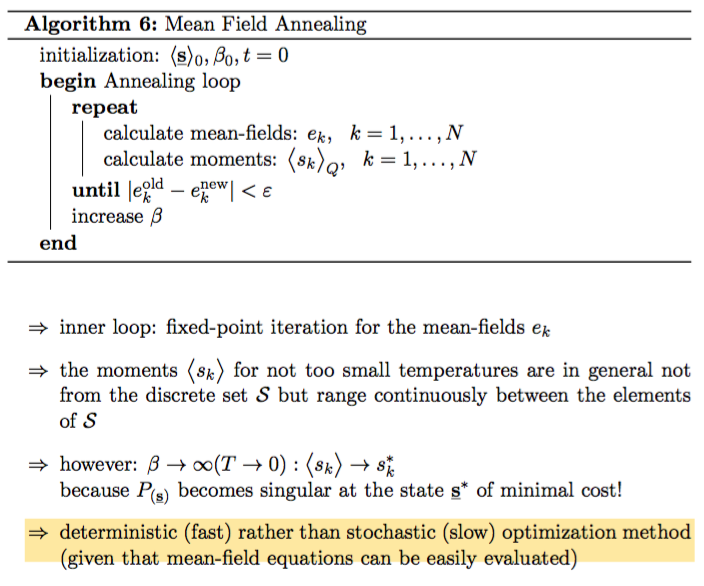
\includegraphics[width=0.5\textwidth]{figures/so-mean-field-algo}
  \caption{Drawn from MI2 course note }
  \label{fig:so-transition-probability}
\end{figure}

\subsubsection{Mean Field for Ising Model}
$\boldsymbol{s}  = \{ s_i \}_{i = 1, .. , N} $ where $s_i \in \mathcal{S} ={-1,1}$ and 
$$E_{(\boldsymbol{s})}  = -\frac{1}{2} \sum_{i,j = 1, i \ne j }^{N}  W_{ij} s_i s_j$$
where $W$ is a real symmetric matric with zero diagonal entries.

\begin{enumerate}
	\item The first moment $\langle s_l \rangle_Q$ can be computed follows : 
	\begin{align*}
\langle s_l \rangle_Q &=		 \frac{ \sum_{s_{l,i} \in s_l} s_{l,i} \exp{ \bigg ( -\beta e_l s_{l,i} \bigg)} }{ \sum_{s_{l,i} \in s_l} \exp{ \bigg ( -\beta e_l s_{l,i} \bigg)} }  \\
&= \frac{  \exp{  ( -\beta e_l  )} - \exp{  ( \beta e_l  )} }{ \exp{  ( -\beta e_l  )}  + \exp{  ( \beta e_l  )}}  \\
&= \tanh ( -\beta e_l )
	\end{align*}
	\item $e_l$ is computed by 
\begin{align*}
0 &=	\frac{\partial}{\partial e_l} \langle E_P \rangle_Q  -   e_l \frac{\partial}{\partial e_l} \langle  s_l \rangle_Q \\
&=	\frac{\partial}{\partial e_l} \bigg \langle -\frac{1}{2} \sum_{i,j = 1, i \ne j }^{N}  W_{ij} s_i s_j \bigg \rangle_Q  -   e_l \frac{\partial}{\partial e_l} \langle  s_l \rangle_Q  \\
&=	-\frac{1}{2} \frac{\partial}{\partial e_l}   \sum_{i,j = 1, i \ne j }^{N}  W_{ij} \langle s_i \rangle_Q \langle s_j  \rangle_Q  -   e_l \frac{\partial}{\partial e_l} \langle  s_l \rangle_Q  \\
&= \sum_{i = 1, i \ne l }^{N}  W_{il} \langle s_i \rangle_Q \frac{\partial}{\partial e_l} \langle s_l  \rangle_Q  -   e_l \frac{\partial}{\partial e_l} \langle  s_l \rangle_Q 
\end{align*}
\end{enumerate}
Hence, 
$$
e_l = \sum_{i = 1, i \ne l }^{N}  W_{il} \langle s_i \rangle_Q
$$